\documentclass[11pt]{article}

%%%%%%%%%%%%%%%%%%%%%%%%%%%%%%%%%%%%%%%%%
% Cleese Assignment
% Structure Specification File
% Version 1.0 (27/5/2018)
%
% This template originates from:
% http://www.LaTeXTemplates.com
%
% Author:
% Vel (vel@LaTeXTemplates.com)
%
% License:
% CC BY-NC-SA 3.0 (http://creativecommons.org/licenses/by-nc-sa/3.0/)
% 
%%%%%%%%%%%%%%%%%%%%%%%%%%%%%%%%%%%%%%%%%

%----------------------------------------------------------------------------------------
%	PACKAGES AND OTHER DOCUMENT CONFIGURATIONS
%----------------------------------------------------------------------------------------

\usepackage{lastpage} % Required to determine the last page number for the footer

\usepackage{graphicx} % Required to insert images

\setlength\parindent{0pt} % Removes all indentation from paragraphs

\usepackage[most]{tcolorbox} % Required for boxes that split across pages

\usepackage{booktabs} % Required for better horizontal rules in tables

\usepackage{listings} % Required for insertion of code

\usepackage{etoolbox} % Required for if statements

%----------------------------------------------------------------------------------------
%	MARGINS
%----------------------------------------------------------------------------------------

\usepackage{geometry} % Required for adjusting page dimensions and margins

\geometry{
	paper=a4paper, % Change to letterpaper for US letter
	top=3cm, % Top margin
	bottom=3cm, % Bottom margin
	left=2.5cm, % Left margin
	right=2.5cm, % Right margin
	headheight=14pt, % Header height
	footskip=1.4cm, % Space from the bottom margin to the baseline of the footer
	headsep=1.2cm, % Space from the top margin to the baseline of the header
	%showframe, % Uncomment to show how the type block is set on the page
}

%----------------------------------------------------------------------------------------
%	FONT
%----------------------------------------------------------------------------------------

\usepackage[utf8]{inputenc} % Required for inputting international characters
\usepackage[T1]{fontenc} % Output font encoding for international characters

\usepackage[sfdefault,light]{roboto} % Use the Roboto font

%----------------------------------------------------------------------------------------
%	HEADERS AND FOOTERS
%----------------------------------------------------------------------------------------

\usepackage{fancyhdr} % Required for customising headers and footers

\pagestyle{fancy} % Enable custom headers and footers

\lhead{\small\assignmentClass\ifdef{\assignmentClassInstructor}{\ (\assignmentClassInstructor):}{}\ \assignmentTitle} % Left header; output the instructor in brackets if one was set
\chead{} % Centre header
\rhead{\small\ifdef{\assignmentAuthorName}{\assignmentAuthorName}{\ifdef{\assignmentDueDate}{\assignmentDueDate}{}}} % Right header; output the author name if one was set, otherwise the due date if that was set

\lfoot{} % Left footer
\cfoot{\small Page\ \thepage\ of\ \pageref{LastPage}} % Centre footer
\rfoot{} % Right footer

\renewcommand\headrulewidth{0.5pt} % Thickness of the header rule

%----------------------------------------------------------------------------------------
%	MODIFY SECTION STYLES
%----------------------------------------------------------------------------------------

\usepackage{titlesec} % Required for modifying sections

%------------------------------------------------
% Section

\titleformat
{\section} % Section type being modified
[block] % Shape type, can be: hang, block, display, runin, leftmargin, rightmargin, drop, wrap, frame
{\Large\bfseries} % Format of the whole section
{\assignmentQuestionName~\thesection} % Format of the section label
{6pt} % Space between the title and label
{} % Code before the label

\titlespacing{\section}{0pt}{0.5\baselineskip}{0.5\baselineskip} % Spacing around section titles, the order is: left, before and after

%------------------------------------------------
% Subsection

\titleformat
{\subsection} % Section type being modified
[block] % Shape type, can be: hang, block, display, runin, leftmargin, rightmargin, drop, wrap, frame
{\itshape} % Format of the whole section
{(\alph{subsection})} % Format of the section label
{4pt} % Space between the title and label
{} % Code before the label

\titlespacing{\subsection}{0pt}{0.5\baselineskip}{0.5\baselineskip} % Spacing around section titles, the order is: left, before and after

\renewcommand\thesubsection{(\alph{subsection})}

%----------------------------------------------------------------------------------------
%	CUSTOM QUESTION COMMANDS/ENVIRONMENTS
%----------------------------------------------------------------------------------------

% Environment to be used for each question in the assignment
\newenvironment{question}{
	\vspace{0.5\baselineskip} % Whitespace before the question
	\section{} % Blank section title (e.g. just Question 2)
	\lfoot{\small\itshape\assignmentQuestionName~\thesection~continued on next page\ldots} % Set the left footer to state the question continues on the next page, this is reset to nothing if it doesn't (below)
}{
	\lfoot{} % Reset the left footer to nothing if the current question does not continue on the next page
}

%------------------------------------------------

% Environment for subquestions, takes 1 argument - the name of the section
\newenvironment{subquestion}[1]{
	\subsection{#1}
}{
}

%------------------------------------------------

% Command to print a question sentence
\newcommand{\questiontext}[1]{
	\textbf{#1}
	\vspace{0.5\baselineskip} % Whitespace afterwards
}

%------------------------------------------------

% Command to print a box that breaks across pages with the question answer
\newcommand{\answer}[1]{
	\begin{tcolorbox}[breakable, enhanced]
		#1
	\end{tcolorbox}
}

%------------------------------------------------

% Command to print a box that breaks across pages with the space for a student to answer
\newcommand{\answerbox}[1]{
	\begin{tcolorbox}[breakable, enhanced]
		\vphantom{L}\vspace{\numexpr #1-1\relax\baselineskip} % \vphantom{L} to provide a typesetting strut with a height for the line, \numexpr to subtract user input by 1 to make it 0-based as this command is
	\end{tcolorbox}
}

%------------------------------------------------

% Command to print an assignment section title to split an assignment into major parts
\newcommand{\assignmentSection}[1]{
	{
		\centering % Centre the section title
		\vspace{2\baselineskip} % Whitespace before the entire section title
		
		\rule{0.8\textwidth}{0.5pt} % Horizontal rule
		
		\vspace{0.75\baselineskip} % Whitespace before the section title
		{\LARGE \MakeUppercase{#1}} % Section title, forced to be uppercase
		
		\rule{0.8\textwidth}{0.5pt} % Horizontal rule
		
		\vspace{\baselineskip} % Whitespace after the entire section title
	}
}

%----------------------------------------------------------------------------------------
%	TITLE PAGE
%----------------------------------------------------------------------------------------

\author{\textbf{\assignmentAuthorName}} % Set the default title page author field
\date{} % Don't use the default title page date field

\title{
	\thispagestyle{empty} % Suppress headers and footers
	\vspace{0.2\textheight} % Whitespace before the title
	\textbf{\assignmentClass:\ \assignmentTitle}\\[-4pt]
	\ifdef{\assignmentDueDate}{{\small Fecha de entrega:\ \assignmentDueDate}\\}{} % If a due date is supplied, output it
	\ifdef{\assignmentClassInstructor}{{\large \textit{\assignmentClassInstructor}}}{} % If an instructor is supplied, output it
	\vspace{0.32\textheight} % Whitespace before the author name
}


\usepackage{amssymb}
\usepackage{enumerate}
\usepackage{graphicx}

\usepackage{listings}
\usepackage{xcolor}

\definecolor{codegreen}{rgb}{0,0.6,0}
\definecolor{codegray}{rgb}{0.5,0.5,0.5}
\definecolor{codepurple}{rgb}{0.58,0,0.82}
\definecolor{backcolour}{rgb}{0.95,0.95,0.92}

\lstdefinestyle{mystyle}{
    backgroundcolor=\color{backcolour},   
    commentstyle=\color{codegreen},
    keywordstyle=\color{orange},
    numberstyle=\tiny\color{codegray},
    stringstyle=\color{cyan},
    basicstyle=\ttfamily\footnotesize,
    breakatwhitespace=false,         
    breaklines=true,                 
    captionpos=b,                    
    keepspaces=true,                 
    numbers=left,                    
    numbersep=5pt,                  
    showspaces=false,                
    showstringspaces=false,
    showtabs=false,                  
    tabsize=4
}

\lstset{style=mystyle}

\graphicspath{ {IMAGES/} }

\newcommand{\assignmentQuestionName}{Pregunta}
\newcommand{\assignmentClass}{Arquitectura de Computadoras}
\newcommand{\assignmentTitle}{Laboratorio\ \#5}

\author{
	Blanco Inca, Felix Nestor \\
	\texttt{felix.blanco@utec.edu.pe}
}

\newcommand{\assignmentClassInstructor}{Jorge Gonzalez Reaño}
\newcommand{\assignmentDueDate}{Jueves,\ Junio\ 14\ 2020}

\begin{document}

\maketitle

\thispagestyle{empty}

\newpage

\begin{question}

\questiontext{ 
	\begin{flushleft}
	Diseñando el diagrama de bloques:
	\end{flushleft}
}

\answer{
	En la \emph{figura 1} podemos observar la forma en la que se decidió la división del ALU, las entradas de este ALU son 2 \textit{inputs} de 32 bits cada uno. Un \textit{Arithmetic Unit} donde se encontrarán las operaciones de adición y substracción. Mientras que en el \textit{Logic Unit} se encontrarán las instrucciones de and, or, xor y nor. Dependiendo del valor de \textit{f0} decidiremos si es un operación en \textit{AU} o en \textit{LU}.
	\begin{center} \textbf{Figura 01}: División del ALU 
		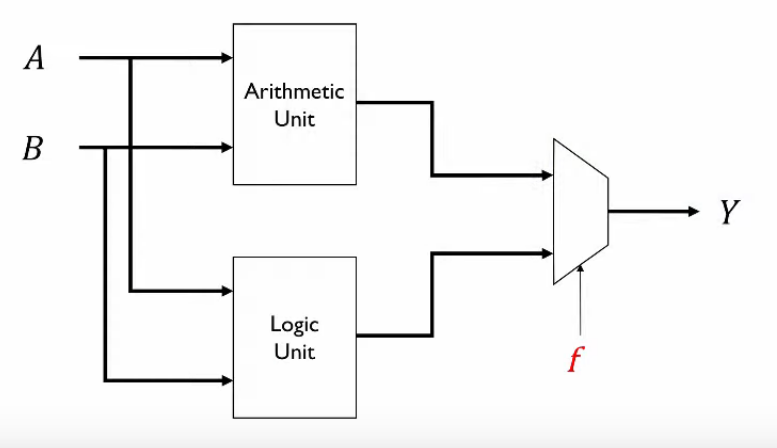
\includegraphics[scale=0.4]{IMAGES_01}
	\end{center}
	Siguiendo con el proceso de diseño, se decide añadir otro multiplexer para que se pueda realizar las operaciones de substracción, pues se necesita que el valor del sustraendo se convierta a \textit{2's complement}. Esta implementación se realiza en ambos inputs para poder realizar ambas operaciones: $A\ -\ B$ y $B\ -\ A$. Dependiendo del valor de \textit{f1} se decide por invertir el input.
	\begin{center} \textbf{Figura 02}: Ainv para operación de substracción 
		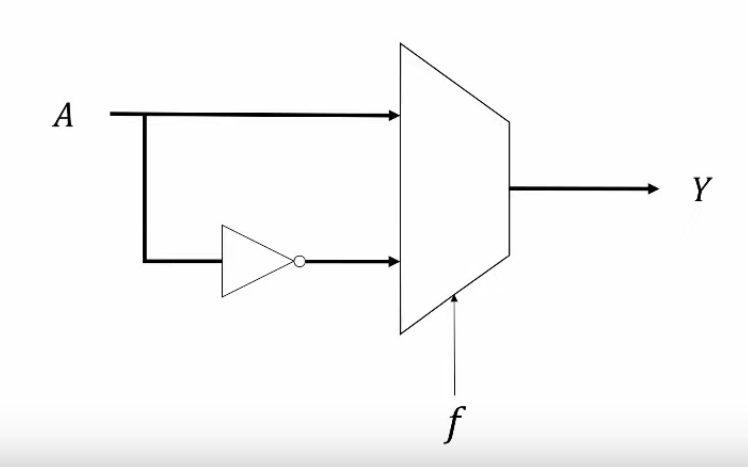
\includegraphics[scale=0.4]{IMAGES_02}
	\end{center}
	A continuacion se muestra la implementación de nuestro diagrama en el programa \textit{Logisim} a fin de verificar la implementación, 
	\begin{center} \textbf{Figura 03}: Logisim, Ainv para operación de sustracción 
		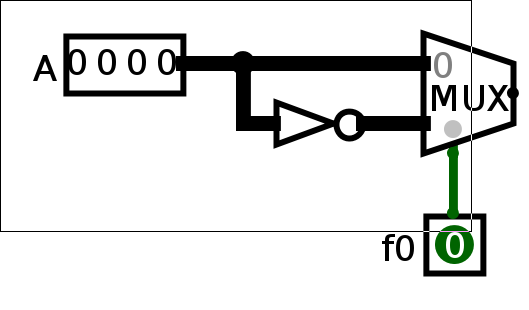
\includegraphics[scale=0.4]{IMAGES_03}
	\end{center}
	Luego de realizar el cambio en el diagrama, podemos ver los cambios. Como se mencionó luego de los 2 inputs de dispuso \textit{2 multiplexers} y \textit{2 not} para invertir el valor del input, dependiendo de los valores de \textit{f0, f1 y f2} se decide los valores de A y B, además de la operación a realizar.
	\begin{center} \textbf{Figura 04}: Diagrama del ALU con los circuitos LU y AU
		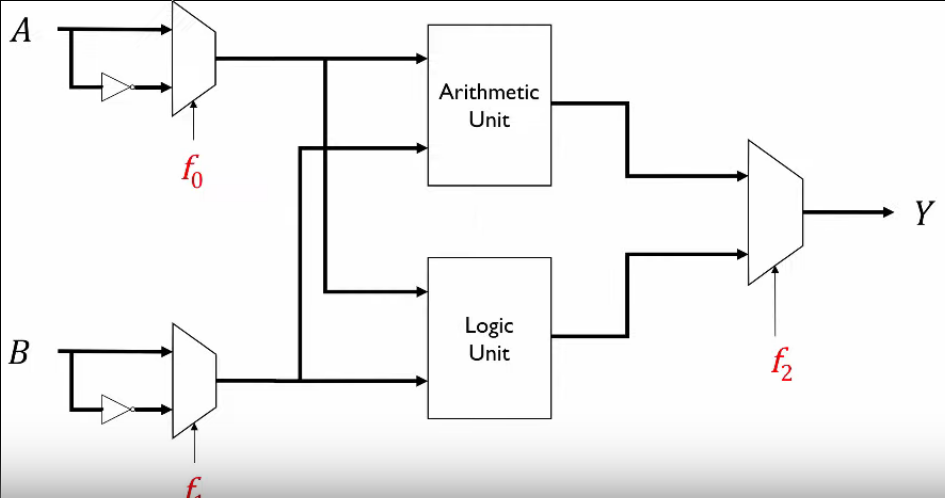
\includegraphics[scale=0.3]{IMAGES_04} 
	\end{center}
	En la \emph{figura 05} se muestra el diseño en Logisim, como se puede apreciar, a ambos circuitos AU y LU ingresan 2 inputs y se retorna el output respectivo, además de los valores de \textit{f1, f2 y f3}.
	\begin{center} \textbf{Figura 05}: Logisim, ALU con los circuitos LU y AUv 
		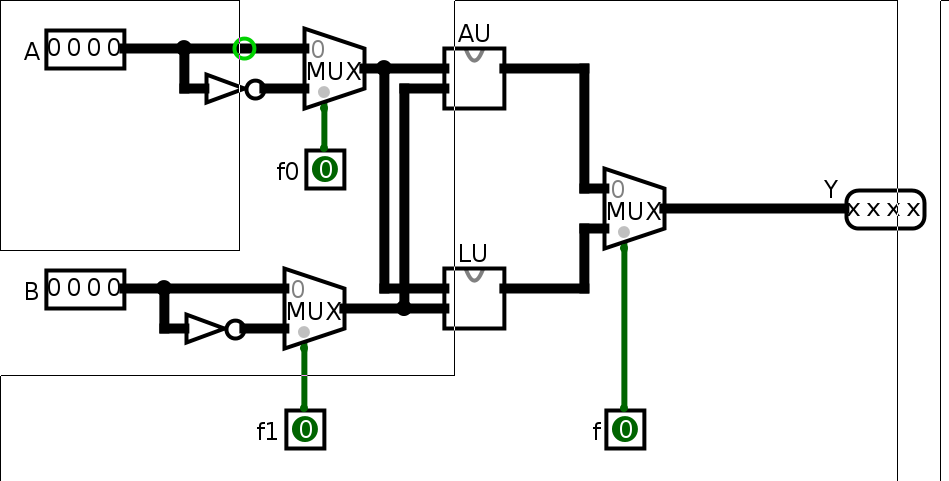
\includegraphics[scale=0.4]{IMAGES_07}
	\end{center}
	Ya tenemos la implementación general del ALU; por lo cual, procederemos a implementar los circuitos \textit{Logic Unit} y \textit{c}. Empezando con el AU, necesitamos un valor de \textit{carry out} que almacene el valor de carry a través de la operación bit a bit. Dependiendo del valor de f se decidirá por lal operaciión a realizar. Para el circuito AU, se utilizarán 2 inputs de 32 bits cada uno y un output del mismo valor.
	\begin{center} \textbf{Figura 06}: Arithmetic Unit, operaciones de adición y substracción 
		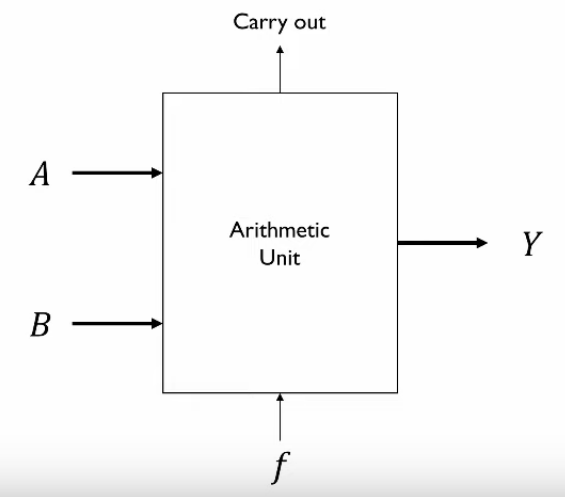
\includegraphics[scale=0.25]{IMAGES_05}
	\end{center}
	En la \emph{figura 07} se ilustra mejor la operación del circuito AU, bit a bit, con la explicación del carry out. Aunque esta es una operación de 4 bits se puede extrapolar a nuestro modelo de 32 bits.
	\begin{center} \textbf{Figura 07}: Explicación de la operación de suma con el carry out 
		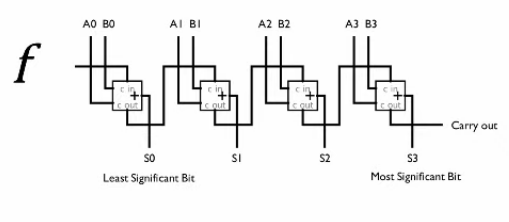
\includegraphics[scale=0.4]{IMAGES_06}
	\end{center}
	En la siguiente figura se muestra el digrama con los valores de entrada de \textit{carry out} y \textit{f2} que necesitaba el circuito AU.
	\begin{center} \textbf{Figura 08}: Diagrama del ALU con valores de carry out y f2 
		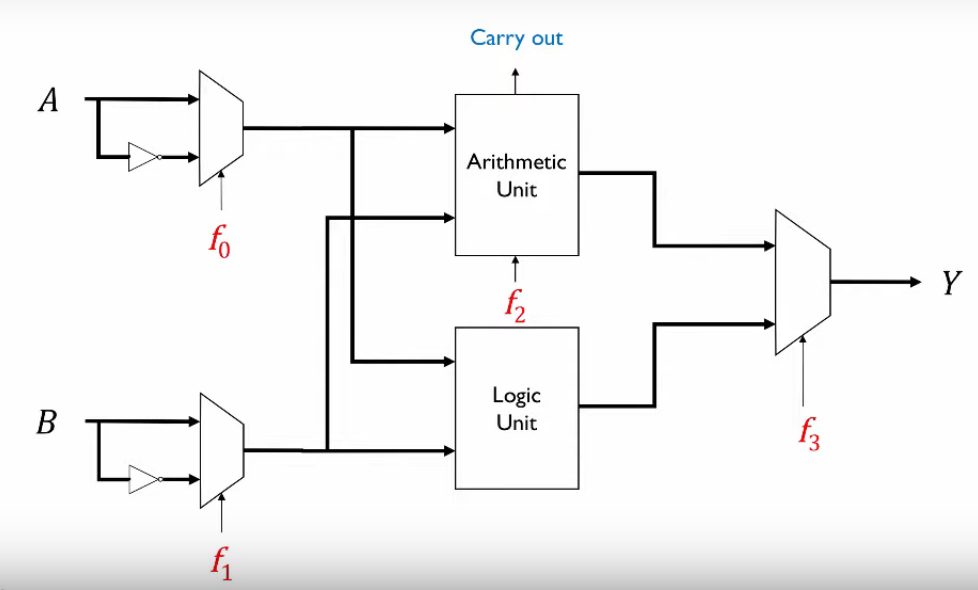
\includegraphics[scale=0.4]{IMAGES_08}
	\end{center}
	Luego de modificar el diagrama del ALU, empezamos a implementarlo en Logisim. Donde le entragamos un input \textit{cin} y se devuelve un output \textit{cout} que sería el valor del carry al final de la operación. Además como se puede apreciar hay un valor de overflow que nos será útil para detectar el signo del valor final. Por otra parte, podemos ver que es una operación de 4 bits la cual extrapolaremos a 32 bits. Para hacer la operación bit a bit, utilizamos un \textit{splitter} que obtendrá el valor de cada bit del input.
	\begin{center} \textbf{Figura 09}: Logisim, ALU con valores de carry out y f2 
		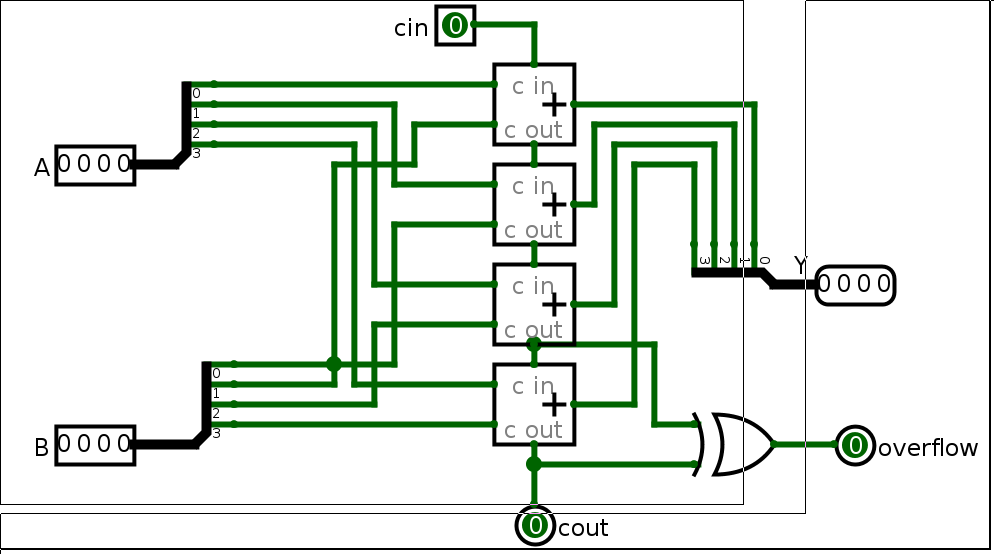
\includegraphics[scale=0.4]{IMAGES_11}
	\end{center}
	En la \emph{figura 10} se detalla para que nos sirve el overflow en el problema de adición y substracción de AU.
	\begin{center} \textbf{Figura 10}: Explicación overflow en la operación
		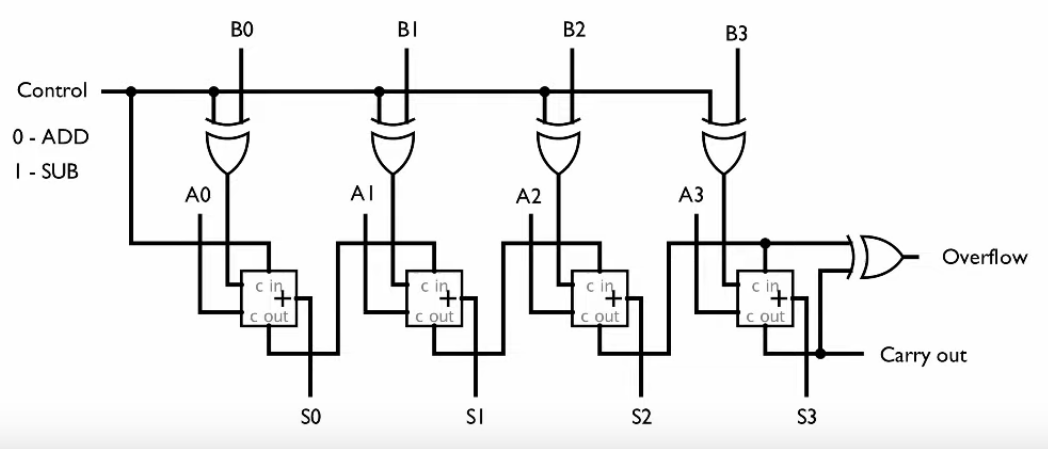
\includegraphics[scale=0.4]{IMAGES_14}
	\end{center}
	Ahora que ya tenemos implementado el AU, procedemos a la implemetación de LU. Al igual que en el AU, se reciben 2 inputs y se devuelve un output. Sin embargo, a diferencia del AU este circuito es controlado por 2 valores en el multiplexer, f2 y f0. Asimismo se describen las compuertas lógicas \textit{and, or, xor y nor}, ambos input tienen un wire que los conecta con cada una de las compuertas y finalmente al multiplexer que decide la operación lógica y retornar el ouput.
	\begin{center} \textbf{Figura 09}: Diagrama del LU, con valores de f2 y f0
		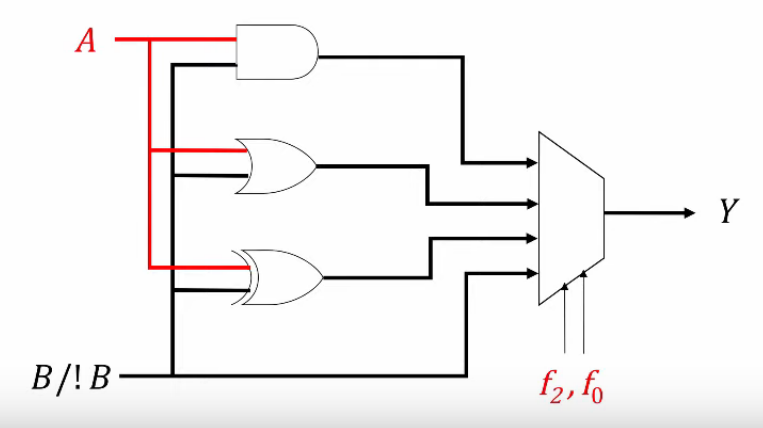
\includegraphics[scale=0.3]{IMAGES_09}
	\end{center}
	A continuación se verá la implementación en Logisim, donde se muestra las compuertas lógicas y los wires a utiliiizar, además del multiplexer y los inputs respectivos.
	\begin{center} \textbf{Figura 10}: Logisim, LU con sus respectivas compuertas lógicas
		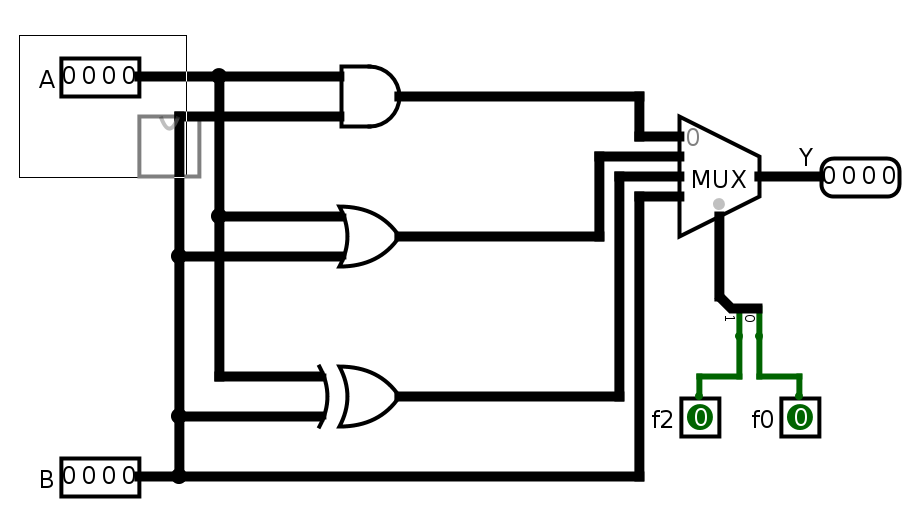
\includegraphics[scale=0.3]{IMAGES_12}
	\end{center}
	Comm se  vio en la anterior explicación es necesario añadir dos input en el diagrama de nuestro circuito LU, en la \emph{figura 11} se puede ver el cambio realizado.
	\begin{center} \textbf{Figura 11}: Diagrama ALU, valores  de f2 y f0 añadidos 
		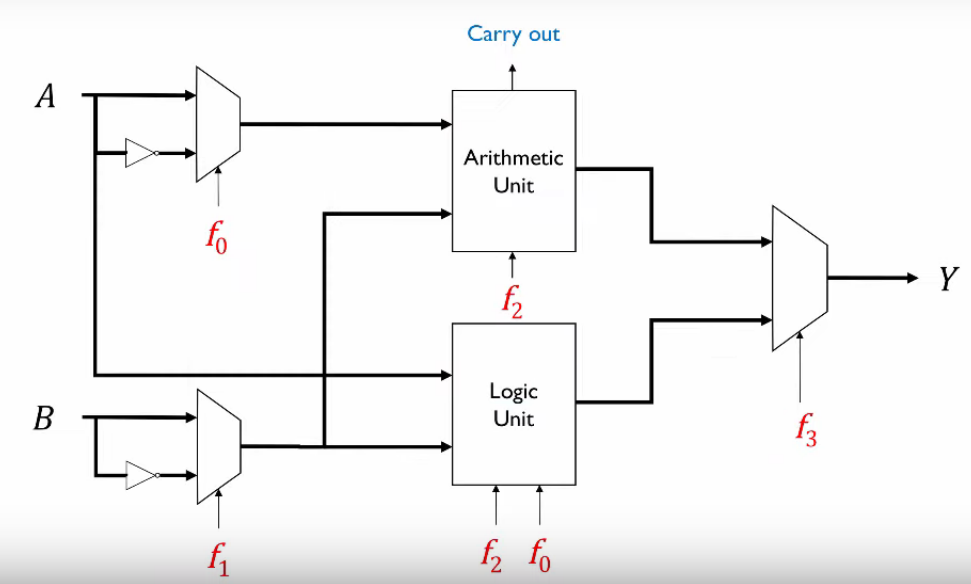
\includegraphics[scale=0.3]{IMAGES_10}
	\end{center}
	Como resultado final, podemos ver nuestro diagrama de ALU en Logisim finalizado con lo valores de \textit{carry in, carry out y overflow}, además, los valores de \textit{f} los agrupamos en un solo inputs de 4 bits que se obtendrán independientemente haciendo uso de un \textit{splitter}. Por otro lado,,  podemos ver 2 nuevos valores de salida Z y N, Z nos indica si el output obtenido es igual a cero, mientras que N nos indica si el output del ALU es negativo.Estos valores como lo son \textit{O, C, Z y N} son \textit{flags} que nos indican situaciones particulares en los resultados obtenidos por el ALU.
	\begin{center} \textbf{Figura 12}: Diagrama ALU con los valores de cin, cout y overflow 
		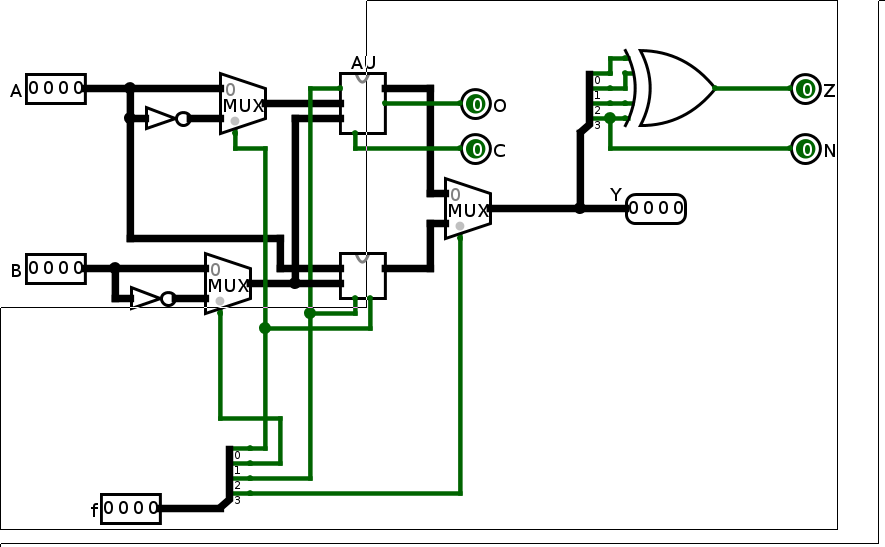
\includegraphics[scale=0.3]{IMAGES_15}
	\end{center}
}

\end{question}

\begin{question}

\questiontext{ 
	\begin{flushleft}
	Implementación en Verilog
	\end{flushleft}
}

\answer{
	
	Para comprobar la funcionalidad del modulo \textit{ALU 32} se decidio el siguiente código.
	\begin{center} \textbf{Listing 01}: Verilog code ALU 32 bits \end{center}
	\begin{flushleft}
	\lstinputlisting[language=Verilog]{alu_32.v}
	\end{flushleft}
}
\answer{
	\begin{flushleft}
	\begin{center} \textbf{Listing 02}: Verilog code ALU 32 bits - Testbench \end{center}
	\begin{flushleft}
		\lstinputlisting[language=Verilog]{alu_32_tb.v}
	\end{flushleft}
	Del testbench se obtuvieron los siguientes resultados, visualizados en GTKWave. Se adjuntan dos capturas:
	En la \emph{figura 13} se presentan los resultados de la una a suma. 
	\begin{center} \textbf{Figura 13}: Resultados TB ALU 32 \newline 
		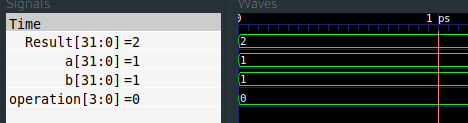
\includegraphics[scale=0.3]{IMAGES_16}
	\end{center}
	Mientras que en la \emph{figura 14} se muestra el resultado de una resta.
	\begin{center} \textbf{Figura 14}: Resultados TB ALU 32  \newline
		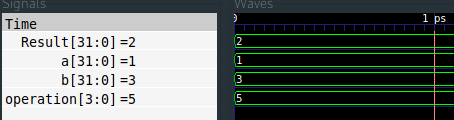
\includegraphics[scale=0.3]{IMAGES_17}
	\end{center}
	Como mejoras a futuro, nos falta implementar un carry out y un overflow. Los cuales son necesarios.
	\end{flushleft}
}
\end{question}

\end{document}
